
\section{The angle of Incidences influence on the headphone transfer function}

\subsection{Purpose}
The purpose of this experiment is to determine if the angle of incidence has any influence on the headphone transfer function and the cancellation path. 

The hypothesis is that the angle on incidence influences both the time delay and magnitude response of the transfer functions.

\subsection{AAU num list}
\begin{table}[H]
	\centering
	\ra{1.3}
	\begin{tabular}{ c c c } \toprule
		{Item}	& {Description} 						& {AAU-no}. \\ \bottomrule 
		1	&	B\&K Head And Torso Simulator "Henry" Type 4128	& 08453		\\
		2	&	B\&K 1'' Condenser Microphone Type 4179 	& 08024\\
		3	&	Sennheiser HD 200	Headphones				& 33379		\\
		4	&	Soundcard RME Fireface 802					& 86838		\\
		5	&	Vision B3565 Computer running simulink		& NaN		\\
		6	&	B\&K Measuring Amplifier Type 2636			& 08717		\\
		7	&	B\&K Sound Calibrator Type 4230				& 08155		\\ 
		8	&	B\&K 1'' Microphone Preamplifier Type 2660	& 08025		\\
		9	&	Genelec speaker								& TBD		\\ 
		10	&	A small microphone to place inside the cup	& TBD\\
		11	& 	B\&K Microphone Power Supply Type 2804		& 07304		\\
		\bottomrule
	\end{tabular}
	\caption{Table over equipment used in test.}
	\label{tab:AngleOfIncideceHP}
\end{table}

\subsection{Diagram}
\begin{figure}[H]
	\centering
	\begin{subfigure}[b]{.4\textwidth}
		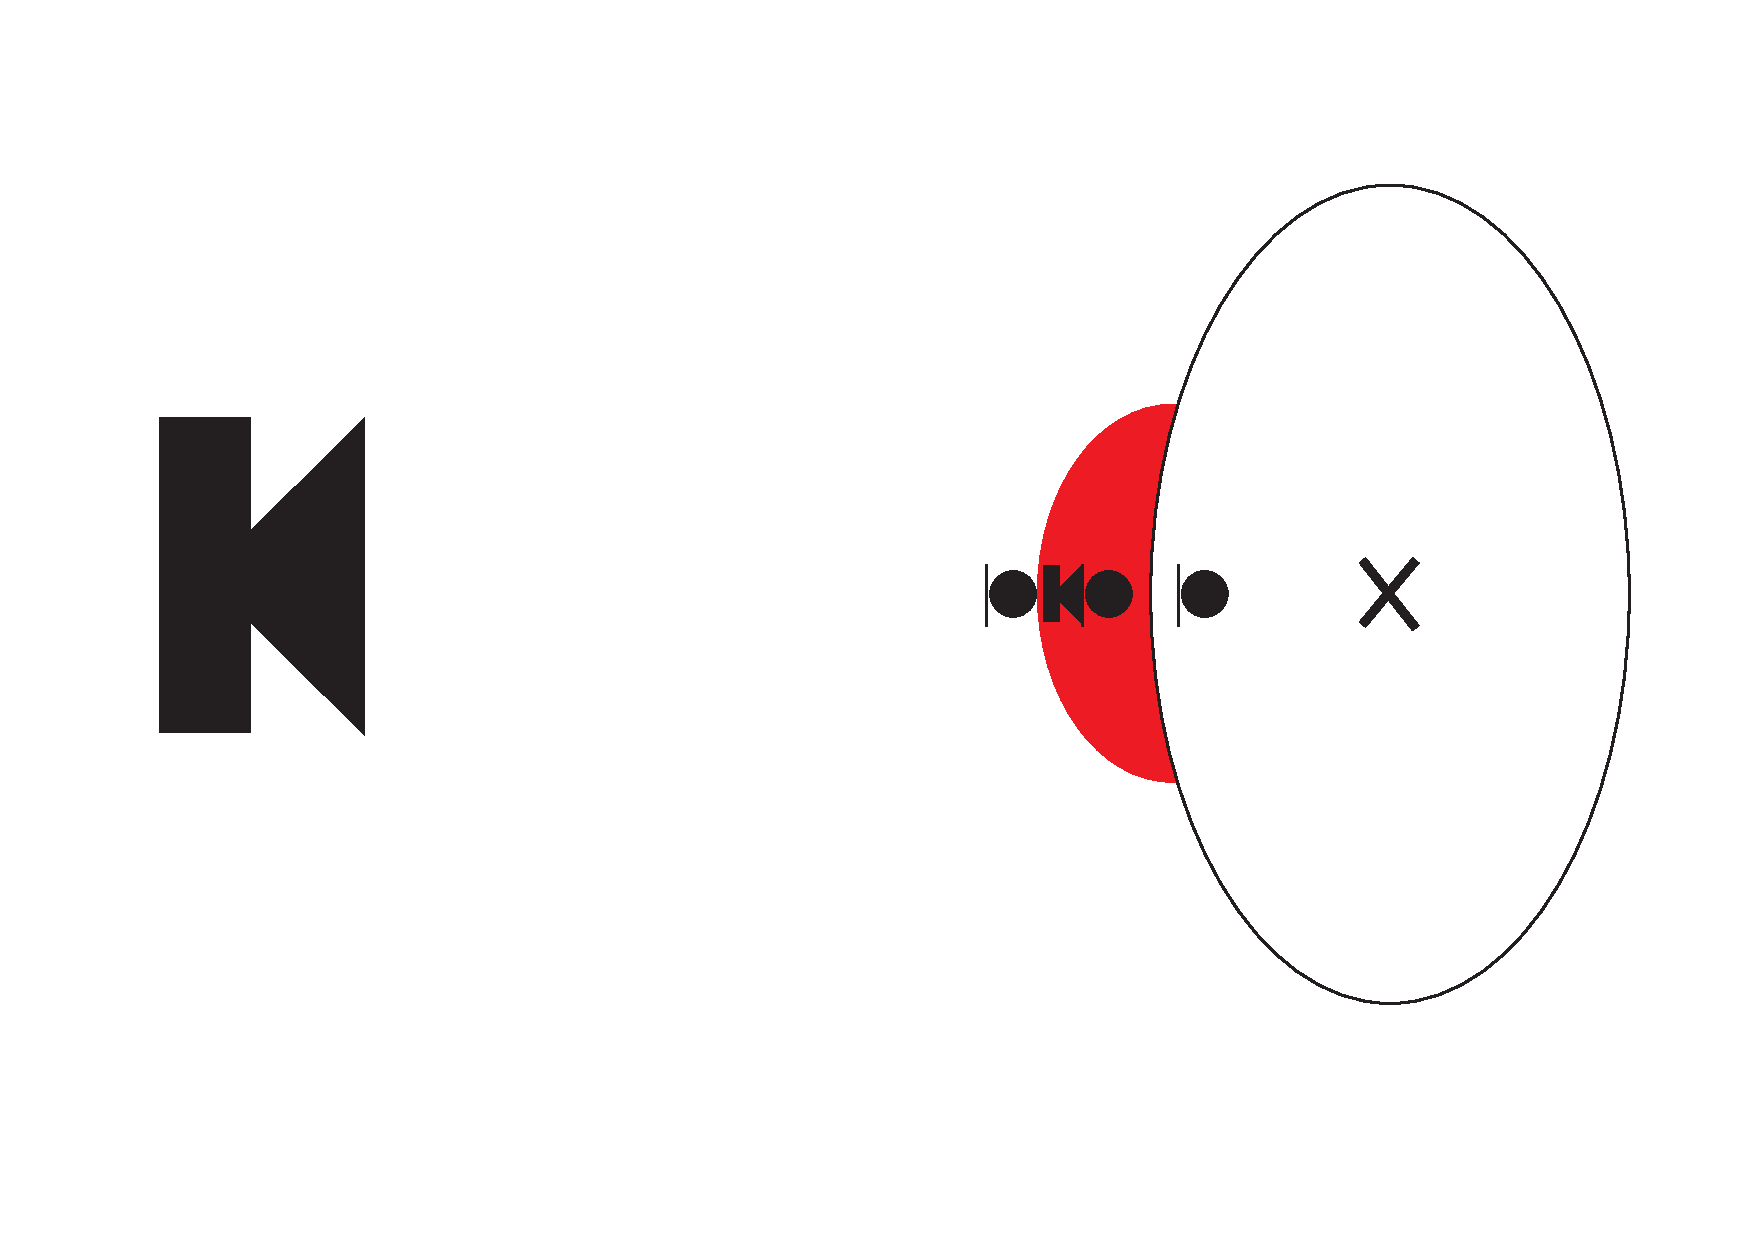
\includegraphics[width=\textwidth]{../Journal/Experiments/AngleOfIncidence/AngleOfIncidenceOnAxis.pdf}
		\caption{On axis}
		\label{fig:AngOgIndOnax}
		\vspace{2ex}
		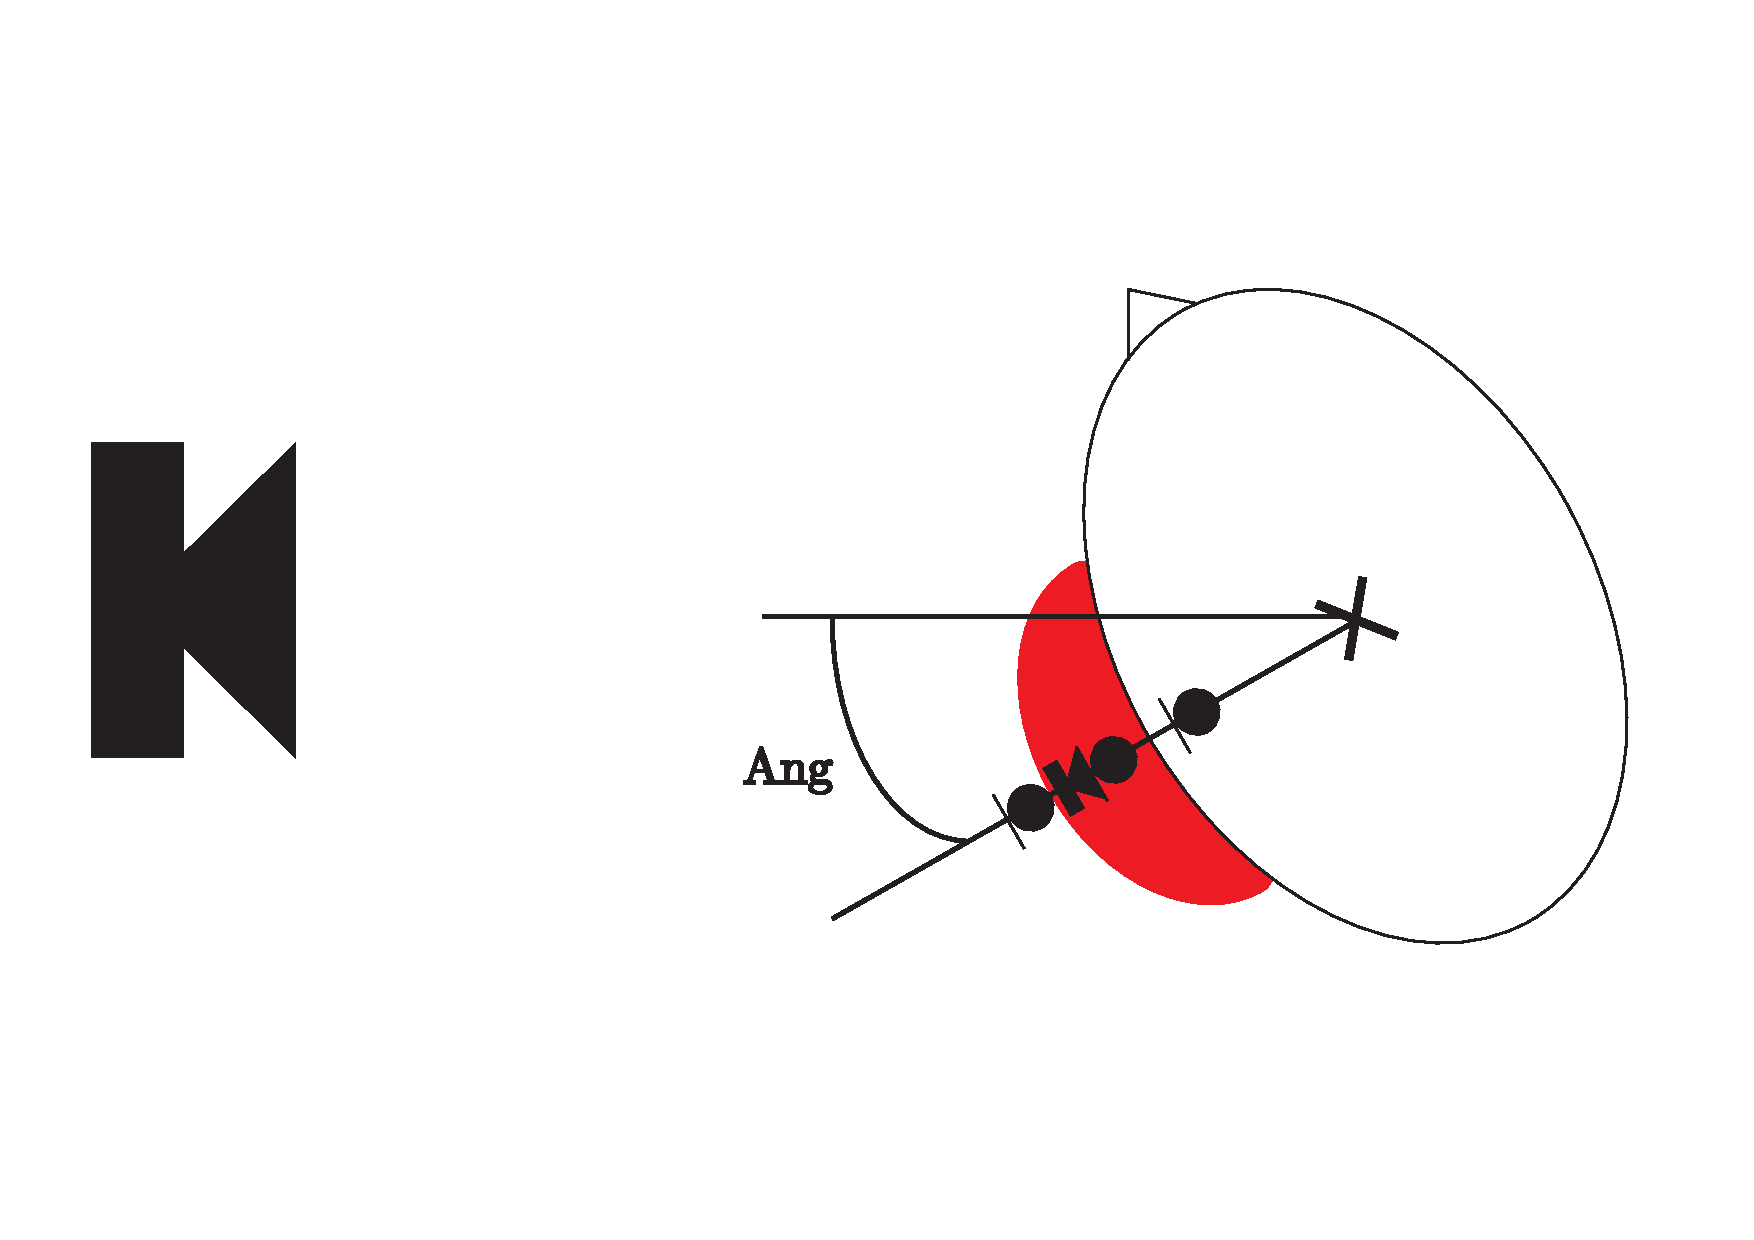
\includegraphics[width=\textwidth]{../Journal/Experiments/AngleOfIncidence/AngleOfIncidenceOffAxis.pdf}
		\caption{Off axis}
		\label{fig:AngOgIndOffax}
	\end{subfigure} 
	\begin{subfigure}[b]{.4\textwidth}
	\centering
	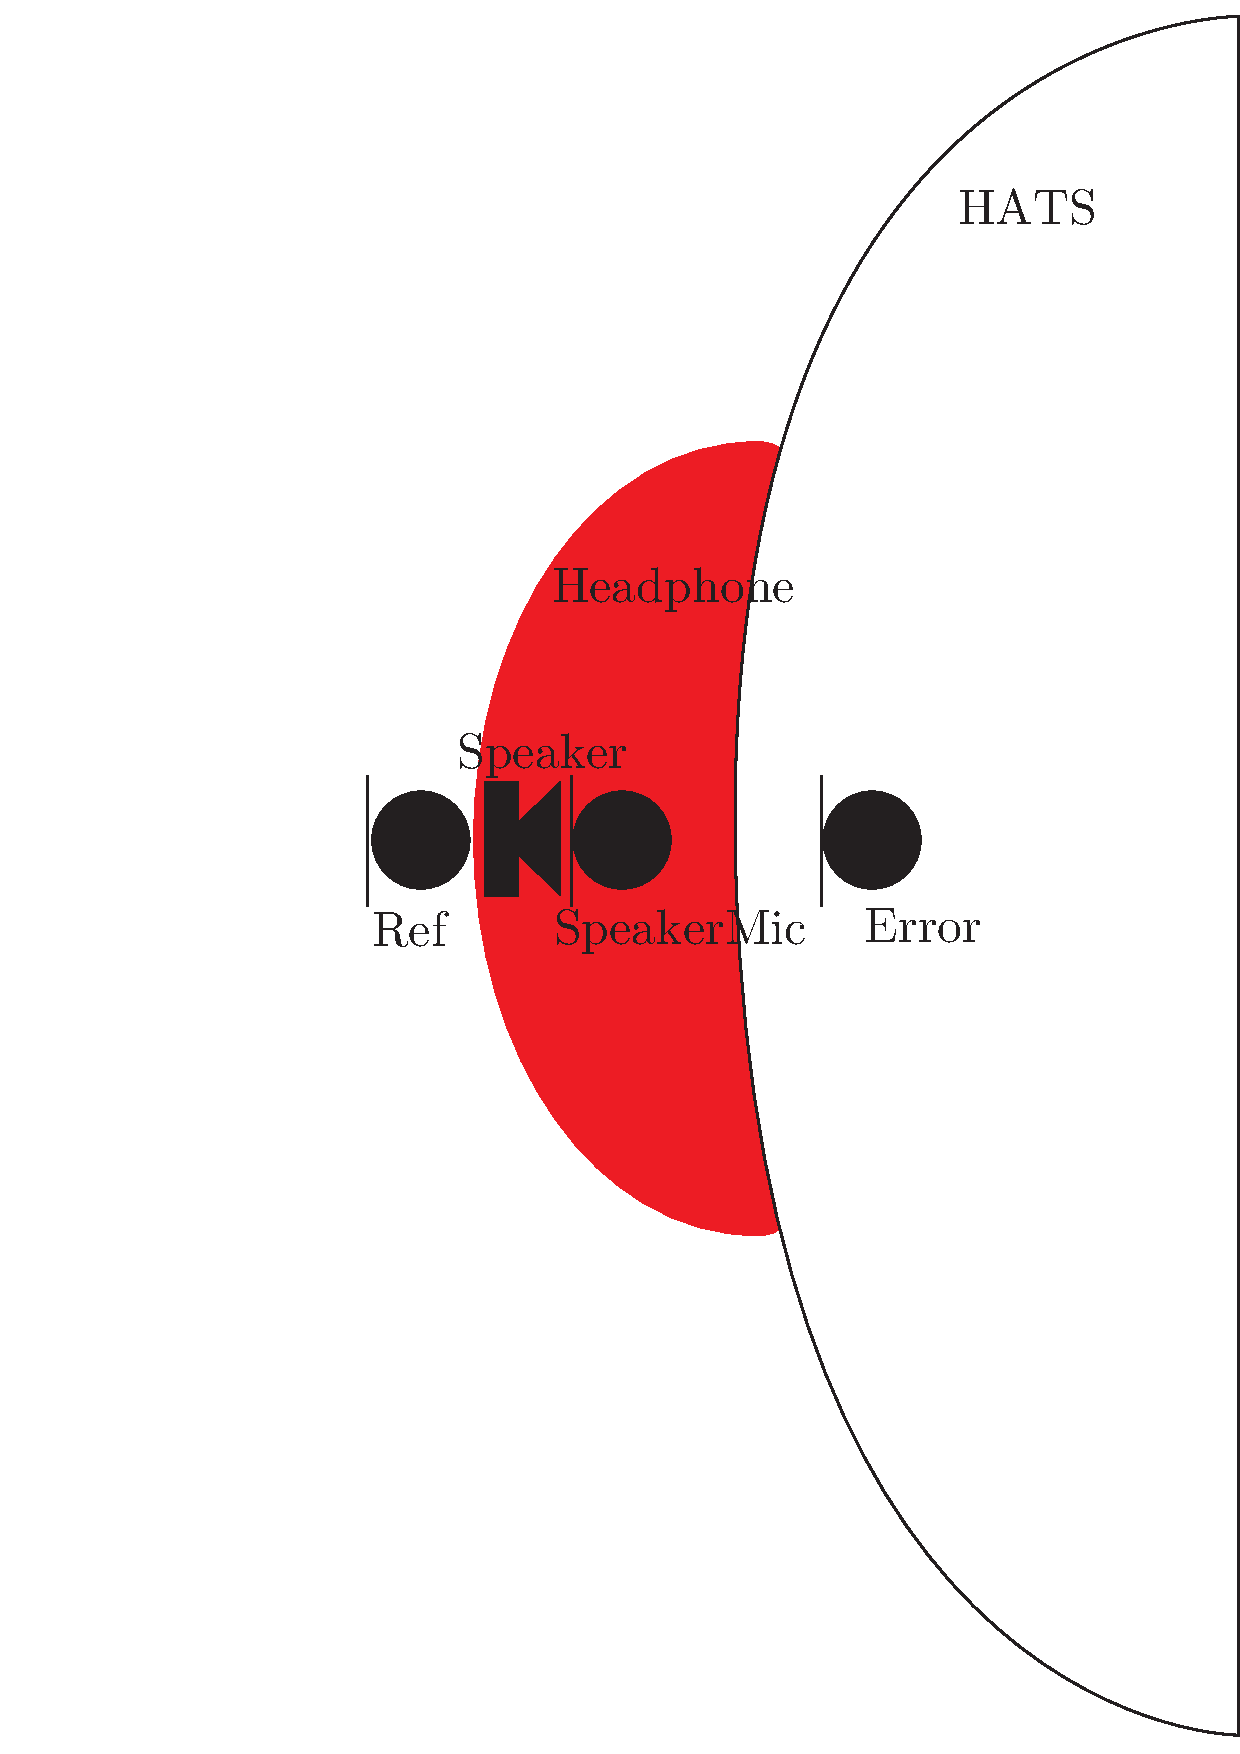
\includegraphics[width=\textwidth]{../Journal/Experiments/AngleOfIncidence/AngleOfIncidenceSchematic.pdf}
	\caption{Placement of microphones}
	\label{fig:AngOgIndMicplace}
\end{subfigure}
	\caption{Placement of microphones and rotation}
	\label{fig:AngleOfIndDiagram}
\end{figure}


\subsection{Settings/Description}
The experiment uses a single speaker to measure angles of incidence. Therefore either the speaker has to be moved around or the HATS will have to be turned to the right angles. \\
Adjusting the angle is done by rotating the HATS around the centre of the HATS leaving the speaker in place. This creates a triangle between the speaker, microphone and inner microphone of the HATS. The baseline of the triangle is from the microphone to the inner microphone, and angle is adjusted according to that line. 
The following Matlab code is used to calculate the angles at which measurements should be performed. The first measurement is performed at a 180\textdegree angle. This determines the length of the baseline (maxI in the code below). After determining the angles of interest can be calculated.  \\
The script is based on two triangles that share a corner, the turning point, and a side to the speaker. The two triangles share the same angle at the turning point. This creates for two equations with two unknowns using the cosine relation and the fact that the side opposite the turning point should have a length "x" in one triangle and "x" + an amount of samples in the other triangle. Using this the angle can  be found.  

\begin{lstlisting} [language=Matlab]
	fs=48000;
	c=342;
	maxI=11;
	metersPrSample=1/(fs/c);
	distM1=0.15; %meters
	% distM2=distM1; %meters
	distSpeaker=1.5; %metersPrSample;
	
	sampledistM1=round(distM1/metersPrSample);
	sampledistM2=round(distM1/metersPrSample)+11;
	sampledistSpeaker=round(distSpeaker/metersPrSample);
	
	i=1:maxI-1;
	
	x= -( sqrt(i.\^2*sampledistM1*sampledistM2 + (sampledistSpeaker\^2 - ...
	sampledistM1*sampledistM2)*(sampledistM1 - sampledistM2)\^2) ...
	- i*sampledistM2)/(sampledistM1 - sampledistM2);
	
	Angle=acosd((sampledistSpeaker\^2+sampledistM2\^2-x.\^2)/ ...
	(2*sampledistM2*sampledistSpeaker));
\end{lstlisting}

\subsection{Control and calibration}
Calibration of the microphone and associated preamplifier is done on the computer using Simulink\textsuperscript{\textregistered}. The following settings are present:
\begin{itemize}
	\item 93.6 dB (-0.4 is subtracted from 94 dB due to adapters) $@$ 1000 Hz is used as calibration signal
	\item Microphone sensitivity is controlled to 110 $m$V/Pa
	\item Measurement amplifier is set to -10 dB default
	\item Calibration signal yields an amplitude of XXX relative to 0 dBFS
	\item  Calibration signal yields a spike of XXX dB SPL at 1000 Hz, which requires a XXX dB SPL adjustment
\end{itemize}
\subsection{Equipment settings}
\begin{itemize}
	\item This experiment is performed with a sampling rate of, $F_{s}$ = 48,000 Hz
	\item The Ref microphone is placed just outside the headset i line with the ear and speaker unit
	\item The SpeakerMic is placed inside the headphone, as close to the speaker unit as possible. 
	\item For item 4 (sound capture card) all gains are set at 0dB		
	\item For item 6 (measuring amplifier):
	\begin{itemize}
		\item "Input Section Gain" is set to +20 dB in proportion to calibration
		\item 22.4 $k$Hz low-pass filter is enabled
		\item 22.4 $k$Hz high-pass filter is enabled 
	\end{itemize}
	\item Item 5 (computer) is set to 0 dBFS
\end{itemize}

\subsection{Picture}

\subsection{Set-up}
\begin{figure}[H]
	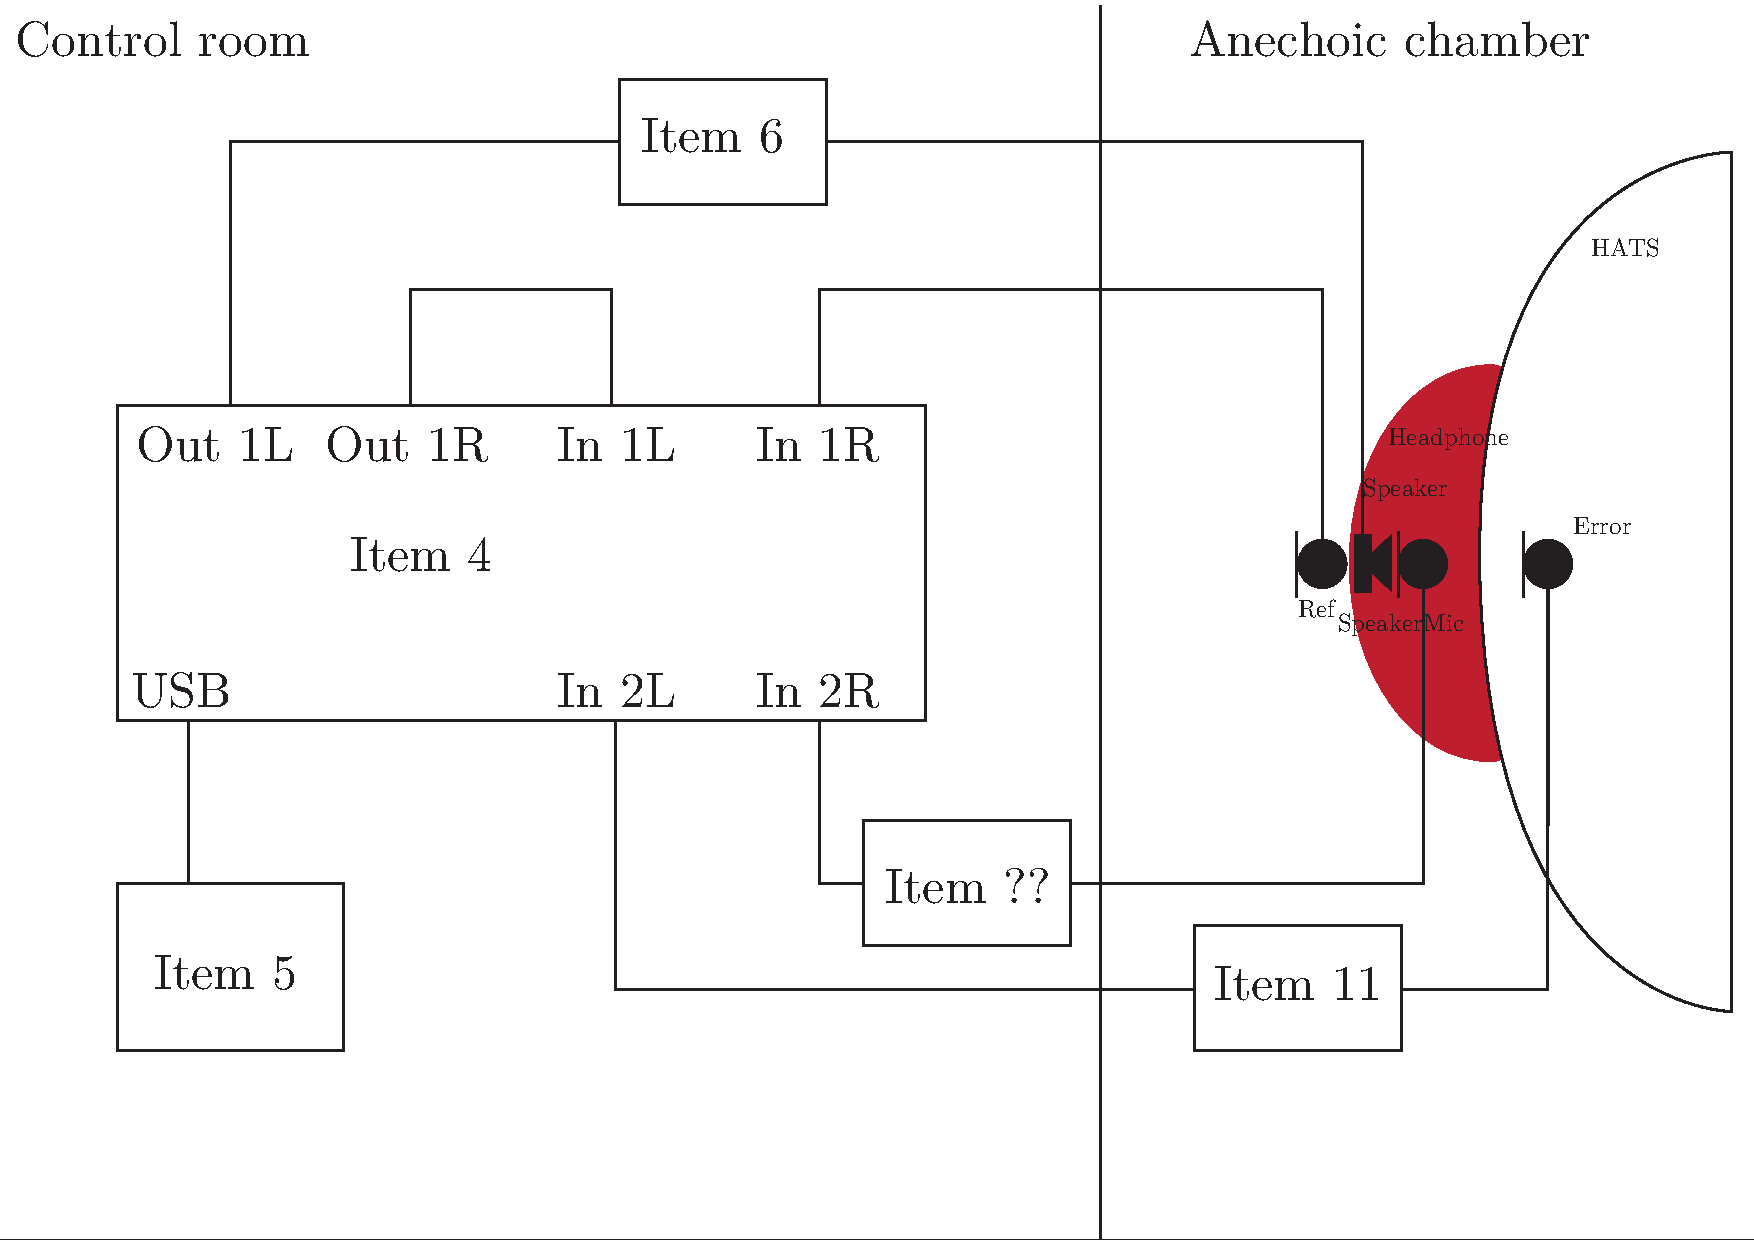
\includegraphics[width=\textwidth]{../Journal/Experiments/AngleOfIncidence/AngleOfIncidenceSetup.pdf}
	\caption{Setup of experiment on angle of incidence}
	\label{Fig:AngleOfIncidenceSetup}
\end{figure}

\subsection{Procedure}
\begin{enumerate}
	\item Open Simulink\textsuperscript{\textregistered} and run file "SimulinkAngleOfIndence.xls"
	\item Run Simulink\textsuperscript{\textregistered} to play "LogChirp.wav" through the speaker
	\item Record and save, and name "Mic[i].wav" and Ref[i].wav" from item 4 onto item 5 \footnote{[i] indicates the iteration of the experiment}
	\begin{itemize}
		\item[] Perform this experiment for all angles given by the Matlab script. 
	\end{itemize}
\end{enumerate}

\subsection{Data Extraction}

\subsection{Analysis}

\subsection{Error Sources}

\subsection{Conclusion}